\documentclass[11pt,DIV12,BCOR0mm,oneside,headings=normal,%
  numbers=noenddot,headsepline,headinclude]{scrreprt}
\usepackage[automark,headsepline]{scrpage2}
\usepackage{scrhack}                % to avoid KOMA-Script warning
\usepackage[utf8]{inputenc}         % UTF8 encoding
%\usepackage[latin1]{inputenc}      % ISO encoding
\usepackage[T1]{fontenc}
\usepackage{txfonts}                % Postscript fonts
\usepackage[ngerman,english]{babel}
\usepackage[fixlanguage]{babelbib}
\usepackage{graphicx}
\usepackage[usenames]{xcolor}
\usepackage{listings}
\usepackage[pdftex]{hyperref}       % provides \url
\usepackage{wallpaper}              % for HsH logo
\usepackage{subfigure}
\usepackage{color}

\definecolor{mygreen}{rgb}{0,0.6,0}
\definecolor{mygray}{rgb}{0.5,0.5,0.5}
\definecolor{mymauve}{rgb}{0.58,0,0.82}

\lstset{ %
	backgroundcolor=\color{white},   % choose the background color; you must add \usepackage{color} or \usepackage{xcolor}; should come as last argument
	basicstyle=\footnotesize,        % the size of the fonts that are used for the code
	breakatwhitespace=false,         % sets if automatic breaks should only happen at whitespace
	breaklines=true,                 % sets automatic line breaking
	captionpos=b,                    % sets the caption-position to bottom
	commentstyle=\color{mygreen},    % comment style
	deletekeywords={...},            % if you want to delete keywords from the given language
	escapeinside={\%*}{*)},          % if you want to add LaTeX within your code
	extendedchars=true,              % lets you use non-ASCII characters; for 8-bits encodings only, does not work with UTF-8
	frame=single,	                   % adds a frame around the code
	keepspaces=true,                 % keeps spaces in text, useful for keeping indentation of code (possibly needs columns=flexible)
	keywordstyle=\color{blue},       % keyword style
	language=Octave,                 % the language of the code
	morekeywords={*,...},           % if you want to add more keywords to the set
	numbers=left,                    % where to put the line-numbers; possible values are (none, left, right)
	numbersep=5pt,                   % how far the line-numbers are from the code
	numberstyle=\tiny\color{mygray}, % the style that is used for the line-numbers
	rulecolor=\color{black},         % if not set, the frame-color may be changed on line-breaks within not-black text (e.g. comments (green here))
	showspaces=false,                % show spaces everywhere adding particular underscores; it overrides 'showstringspaces'
	showstringspaces=false,          % underline spaces within strings only
	showtabs=false,                  % show tabs within strings adding particular underscores
	stepnumber=2,                    % the step between two line-numbers. If it's 1, each line will be numbered
	stringstyle=\color{mymauve},     % string literal style
	tabsize=2,	                   % sets default tabsize to 2 spaces caption instead of title
}

% ---------------------------------------------------------

% package configuration
\KOMAoptions{headinclude}       % for scrpage2
\lstset{numbers=none,showstringspaces=false,language=Java,%
  basicstyle=\ttfamily,frame=single,rulecolor=\color{gray}}
\hypersetup{linkcolor=black,pdfborder=0 0 0}

% layout
\tolerance=2000                 % avoid overfull hboxes
\frenchspacing                  % no extra space after full stops

% ---------------------------------------------------------

\begin{document}

\selectlanguage{english}
\selectbiblanguage{english}

% title page
\thispagestyle{empty}
%\cleardoublepage
\pagenumbering{roman}

\begin{center}
  \vspace*{4\baselineskip}
  {\sffamily\bfseries\LARGE
    React Domain Specific Language\par}
  
  \vspace*{4\baselineskip}
  {\Large }

  \vfill
  {\Large }
  \begin{figure}[htb!]
  	\centerline{
\includegraphics[width=0.8\textwidth]{resources/react-logo.png}}
  \end{figure}
\textbf{} \\
Simplify something simple \\
  
  
  \vspace*{4\baselineskip}
  {\Large \par}
  
  \vspace*{4\baselineskip}
  {\Large 15.\,12.\,2016}
  
  \vspace*{4\baselineskip}
\end{center}


{\huge\textbf{Written by}} \\
\\
\\
\textbf{} \\
Simon Meyer \\
simon.meyer@stud.hs-hannover.de \\
\\
\\
\textbf{} \\
Haminou Mohammed \\
haminou.mohammed@stud.hs-hannover.de \\
\\
\\
\textbf{} \\
Sascha Becker \\
s.becker@wertarbyte.com \\
\\
\\
\\
\\


\tableofcontents    % Table of Contents

%\listoftables       % Tabellenverzeichnis

% main text
\newpage
\pagenumbering{arabic}
\chapter{Introduction}
Javascript is growing rapid fast in mobile web development, server architectures, rest services, desktop cross plattform apps and microservices with the help of nodejs. On top of that every developer can choose which frontend platform is the best choice. React is developed from facebook and provides dynamic DOM manipulation without the need of reloading the complete DOM on every change.

Beside that react has a huge community bas for additional custom components and active issue tracking. Definitely something you should keep an eye on.

\section{Structure}
Every react component follows the same structure. Define your needed imports of react base code and additional components you want your component to use.

Define the default export name and what exactly should be exported. Normally it is your component for sure. A simple code example could look like this:

\begin{lstlisting}
import React, { Component, PropTypes } from 'react'
import { Paper, RaisedButton, TextField } from 'material-ui'

export default class TestName extends Component {
	render() {
		return (
			<Paper style={{ width: 300 }}>
				<TextField
					hintText="Benutzername"
					style={{ float: 'left' }}
				/>
				<TextField
					hintText="Passwort"
					style={{ float: 'middle' }}
				/>
				<RaisedButton
					label="Login"
					style={{ float: 'right' }}
				/>
			</Paper>
		)
	}
}
\end{lstlisting}

\section{UI}
The rendered code above will look like this:
  \begin{figure}[htb!]
	\centerline{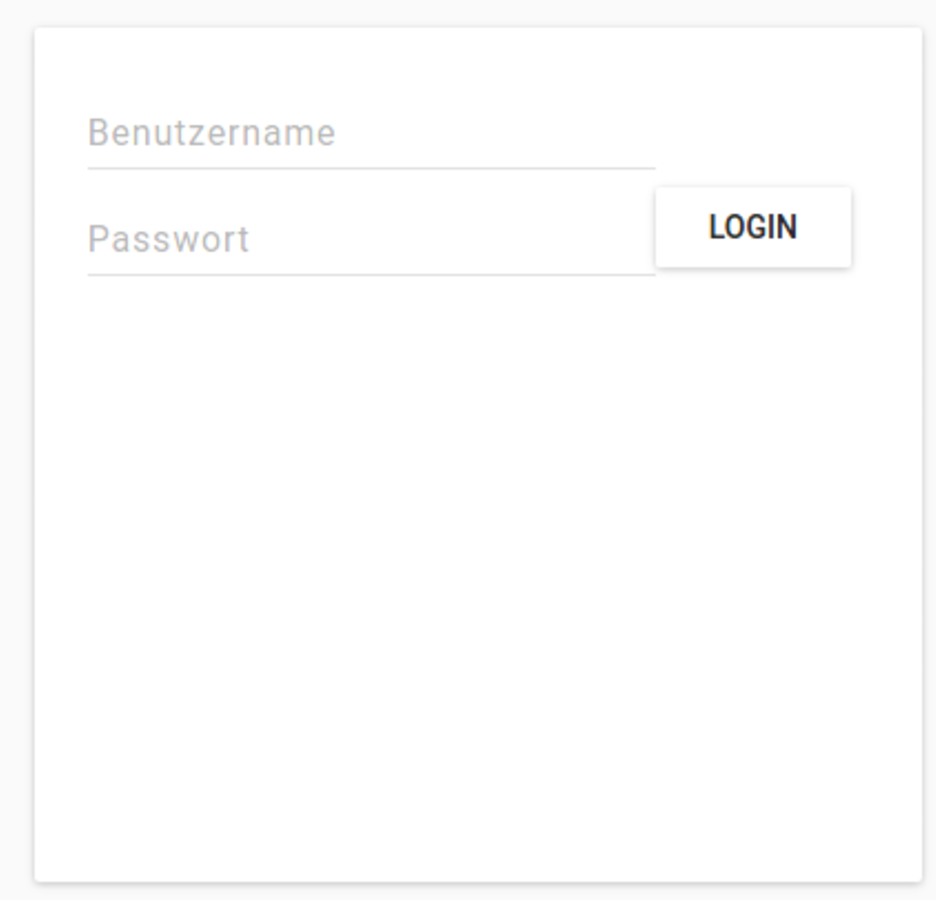
\includegraphics[width=0.8\textwidth]{resources/preview.png}}
\end{figure}
\chapter{Domain Specific Model}
Our model focuses on generating one react component class object. As an example we take a simple paper element which holds two text fields and a button. The needed code looks like this.

\begin{lstlisting}
Class TestName

Component Paper

TextField t1
.hintText="Benutzername"
.style=" float: 'left "

TextField t2
.hintText="Passwort"
.style=" float: 'middle "

Button b1
.label="Login"
.style=" float: 'right "

\end{lstlisting}

First we'll define our react component class name 'TextName'. This identifies our object in a global webapp and provides an import name for incode use. Then we define the root component of this react component. A react component can only return exactly one component. In this case we chose a paper element with 'Component Paper'.

After that we define various other components which get embedded in our root element, the paper component. In this case our textfields get some additional attributes for hinttext and css styling via the '.style' snippet.


\chapter{Grammar}
Our DSM starts with the Model, which contains many Classes. This Classes have a name and null to many materials. The Material can be a Component, a Button or a TextField. If the Material is a Component, it is embedding other Materials. To differentiate between the Attributes of the Materials there is a Property for each Material (ButtonProperty, TextFieldProperty).

\begin{lstlisting}
Model:
root+=Class*
;

Class:	
'Class' name=ID properties+=Material*
;

Material:
Component | Button | TextField
;

Component:
'Component' name=ID
;

Button:
'Button' name=ID properties+=ButtonProperty*
;

ButtonProperty:
Label | ButtonStyle
;

Label:
'.label=' attribute=STRING
;

ButtonStyle:
'.style=' buttonStyle=STRING
;

TextFieldStyle:
'.style=' textfieldStyle=STRING
;

TextField:
'TextField' name=ID properties+=TextFieldProperty*
;

TextFieldProperty:
HintText | TextFieldStyle
;

HintText:
'.hintText=' attribute=STRING
;
\end{lstlisting}

\chapter{Generator}
In the main template the doGenerate Method is creating a new class with ".java" ending for each 'Class' in the Model and will therefore execute the generateComponent Method. In the generateComponent() we iterate through all Materials and creating the Components. The determineElement() in the Component Generation specify the Material and creates the Material with its Attributes.

\lstinputlisting[language=Java]{../src/MyDslGenerator.xtend}

\addcontentsline{toc}{chapter}{Bibliography}
\renewcommand{\btxfnamespaceshort}{\,}

\end{document}
